\documentclass[10pt]{beamer}
\usepackage{bm,booktabs,float,multirow,tabularx}
\usetheme{AnnArbor}
\begin{document}
\title{Design of Integrated Microrobotic Fish}
\subtitle{Presentation 5 - COMSOL Simulation (3D Partial)}
\author{Yihua Liu}
\institute{UM-SJTU Joint Institute}
\date{March 22, 2021}
\maketitle
\begin{frame}{Contents}
    \tableofcontents
\end{frame}
\section{COMSOL Simulation (3D)}
\begin{frame}{COMSOL Simulation (3D)}{Parameters}
    \begin{table}
        \begin{tabular}{|c|c|c|c|}
            \hline
            Name&Expression&Value&Description\\
            \hline
            \multirow{2}{*}{sigma\_KCL}&\multirow{2}{*}{2.1*10\textasciicircum(-3)\lbrack S/m\rbrack}&\multirow{2}{*}{0.0021 S/m}&Conductivity of\\
            &&&the KCL solution\\
            \hline
            c0&1.4[mol/m\textasciicircum3]&1.4 $\mathrm{mol/m^3}$&Initial concentration\\
            \hline
            \multirow{2}{*}{eps\_r}&\multirow{2}{*}{80.2}&\multirow{2}{*}{80.2}&Relative permittivity\\
            &&&of the fluid\\
            \hline
            t&0[s]&0 s&Start time\\
            \hline
            V0&0.1[V]&0.1 V&Applied voltage\\
            \hline
            \multirow{2}{*}{omega}&\multirow{2}{*}{2*pi[rad]*1000[Hz]}&\multirow{2}{*}{6283.2 Hz}&Frequency of the\\
            &&&applied potential\\
            \hline
            D&1e-11[m\textasciicircum2/s]&1E-11 m\textasciicircum/2s&Sample ion diffusivity\\
            \hline
            zeta&-0.1[V]&-0.1 V&Zeta potential\\
            \hline
            U0&0.001[mm/s]&1E-6 m/s&Average velocity\\
            \hline
        \end{tabular}
    \end{table}
\end{frame}
\begin{frame}{Component}{Geometry}
    \begin{figure}[H]
        \centering
        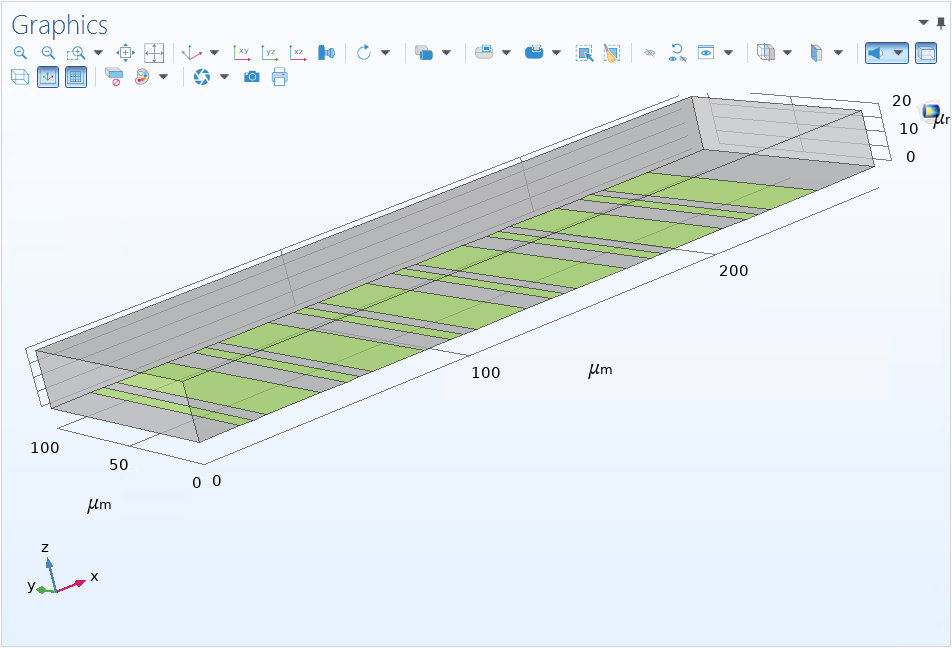
\includegraphics[width=0.8\textwidth]{1.png}
    \end{figure}
\end{frame}
\begin{frame}{Component}{Material}
    \begin{columns}[onlytextwidth]
        \begin{column}{0.5\textwidth}
            KCL [liquid] (mat1)
            \begin{figure}[H]
                \centering
                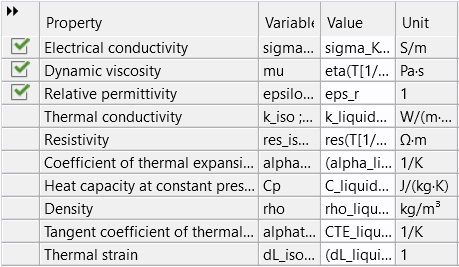
\includegraphics[width=0.9\columnwidth]{2.png}
            \end{figure}
        \end{column}
        \begin{column}{0.5\textwidth}
            Gold [solid] (mat2)
            \begin{figure}[H]
                \centering
                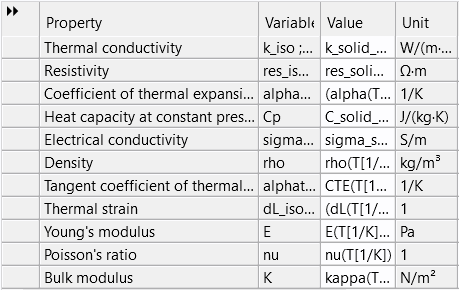
\includegraphics[width=0.9\columnwidth]{3.png}
            \end{figure}
        \end{column}
    \end{columns}
\end{frame}
\begin{frame}{Component}{Electric Currents \textit{ec}}
    \begin{columns}[onlytextwidth]
        \begin{column}{0.5\textwidth}
            small electrodes
            \begin{figure}[H]
                \centering
                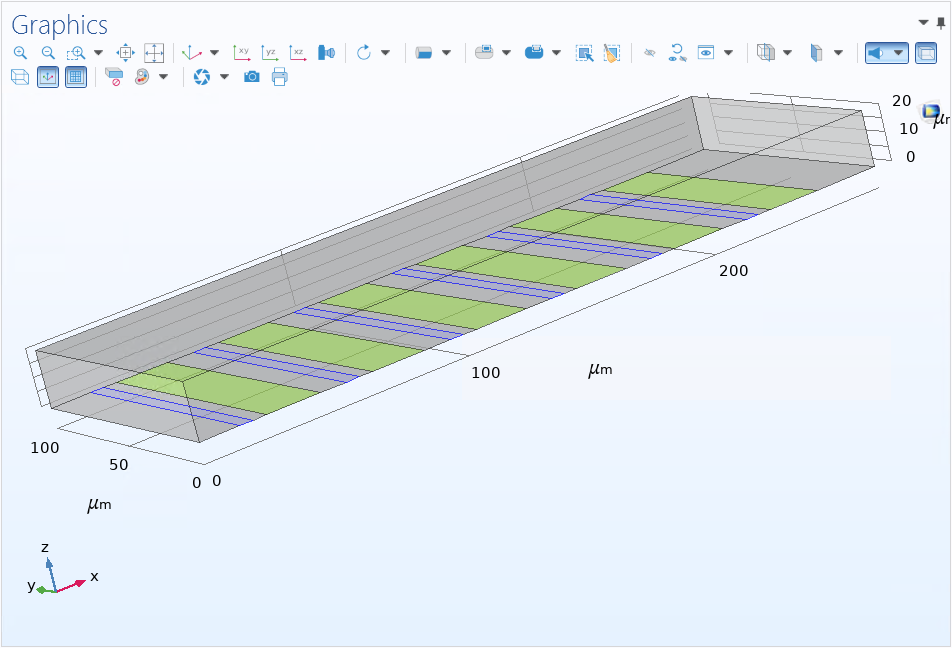
\includegraphics[width=0.9\columnwidth]{4.png}
            \end{figure}
        \end{column}
        \begin{column}{0.5\textwidth}
            large electrodes
            \begin{figure}[H]
                \centering
                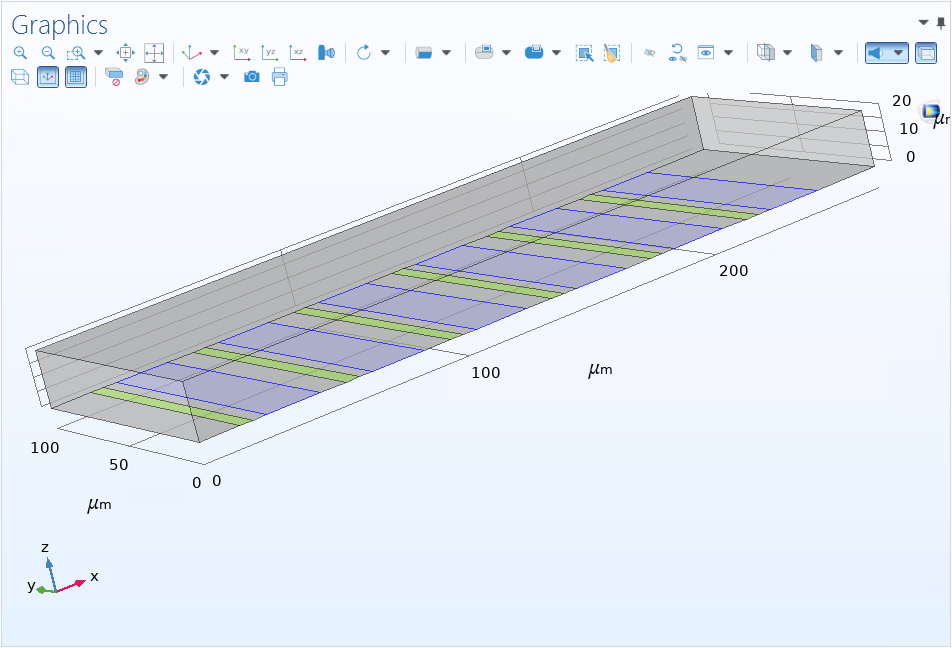
\includegraphics[width=0.9\columnwidth]{5.png}
            \end{figure}
        \end{column}
    \end{columns}
\end{frame}
\begin{frame}{Component}{Transport of Diluted Species \textit{tds}}
    \begin{columns}[onlytextwidth]
        \begin{column}{0.5\textwidth}
            Concentration 1
            \begin{figure}[H]
                \centering
                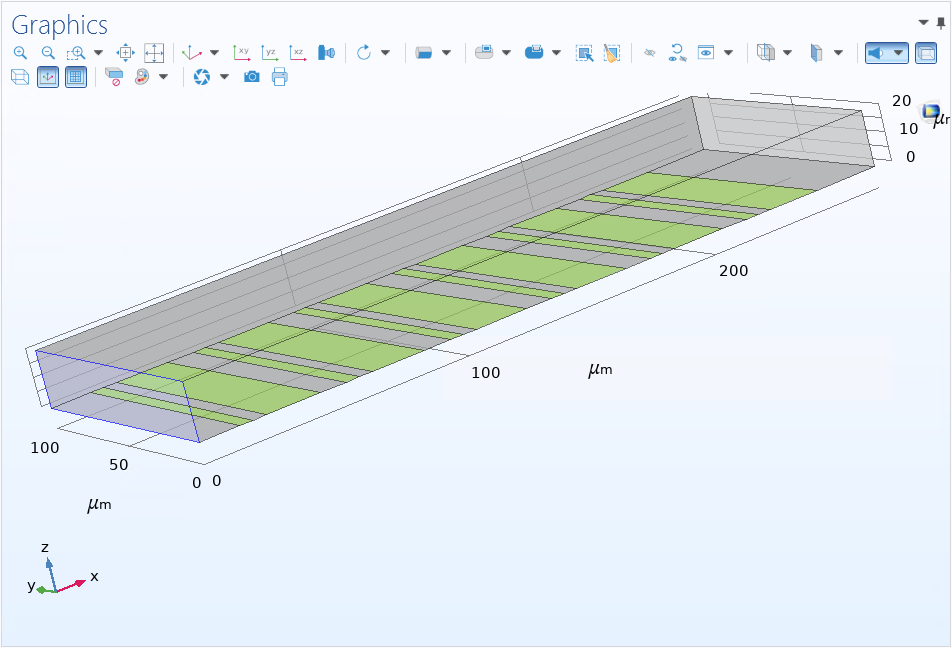
\includegraphics[width=0.9\columnwidth]{6.png}
            \end{figure}
        \end{column}
        \begin{column}{0.5\textwidth}
            Outflow 1
            \begin{figure}[H]
                \centering
                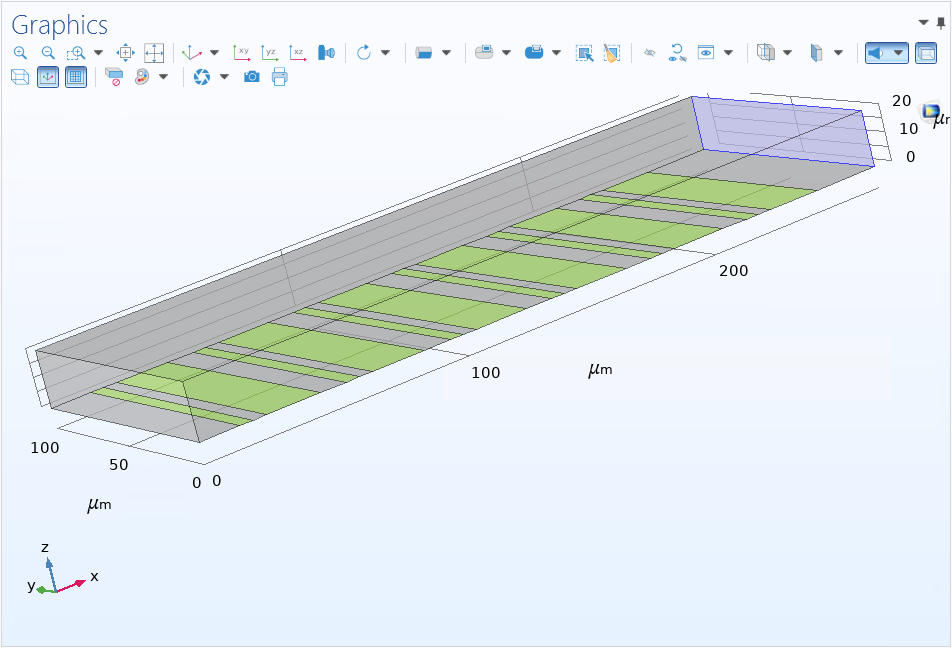
\includegraphics[width=0.9\columnwidth]{7.png}
            \end{figure}
        \end{column}
    \end{columns}
\end{frame}
\begin{frame}{Component}{Creeping Flow \textit{spf}}
    \begin{columns}[onlytextwidth]
        \begin{column}{0.5\textwidth}
            Inlet 1
            \begin{figure}[H]
                \centering
                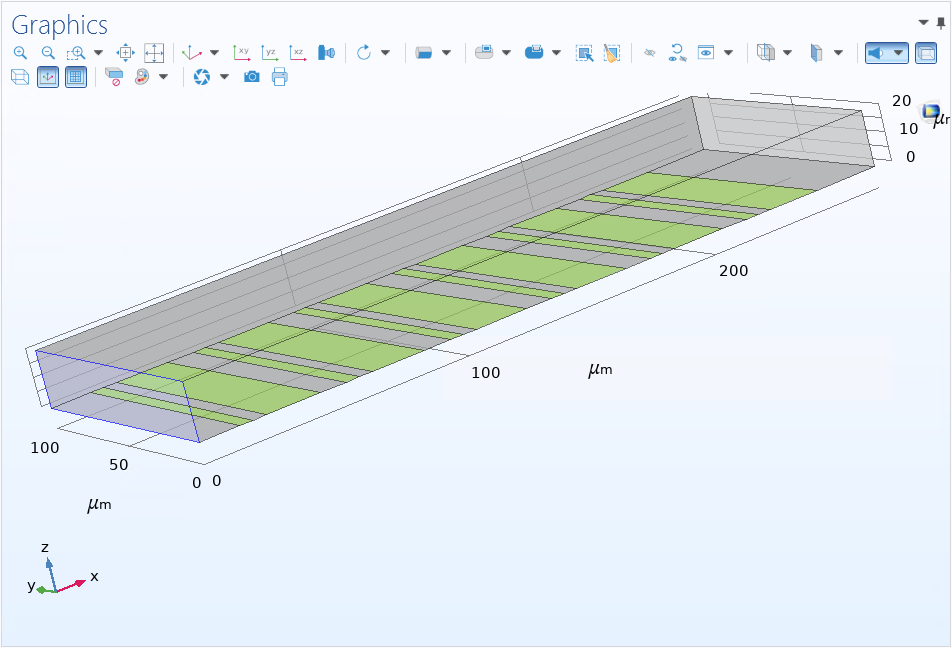
\includegraphics[width=0.9\columnwidth]{6.png}
            \end{figure}
        \end{column}
        \begin{column}{0.5\textwidth}
            Outlet 1
            \begin{figure}[H]
                \centering
                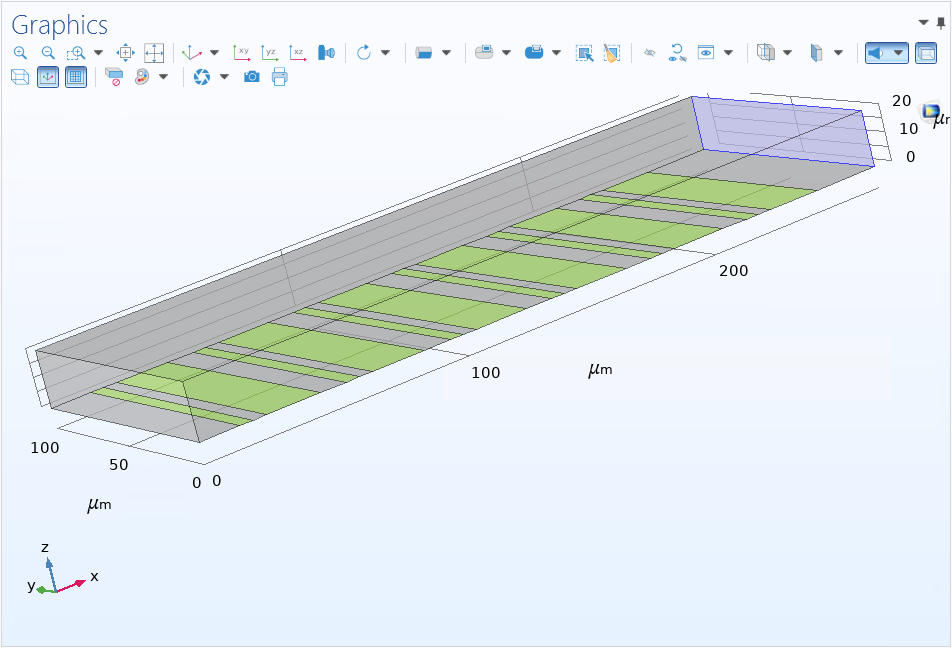
\includegraphics[width=0.9\columnwidth]{7.png}
            \end{figure}
        \end{column}
    \end{columns}
\end{frame}
\begin{frame}{Component}{Mesh}
    Free Tetrahedral 1
    \begin{figure}[H]
        \centering
        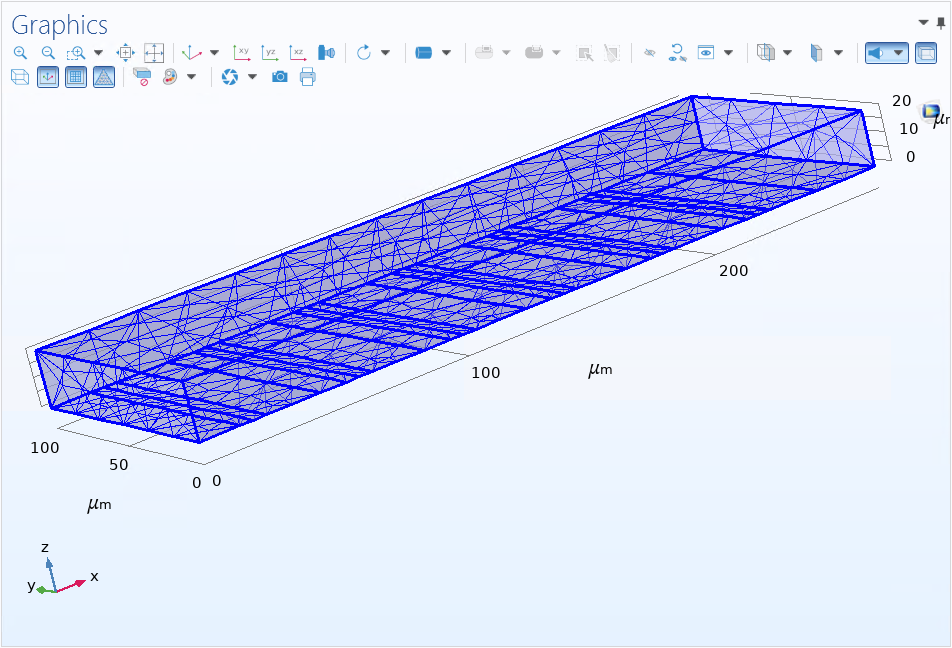
\includegraphics[width=0.8\textwidth]{8.png}
    \end{figure}
\end{frame}
\begin{frame}{Result}
    \begin{figure}[H]
        \centering
        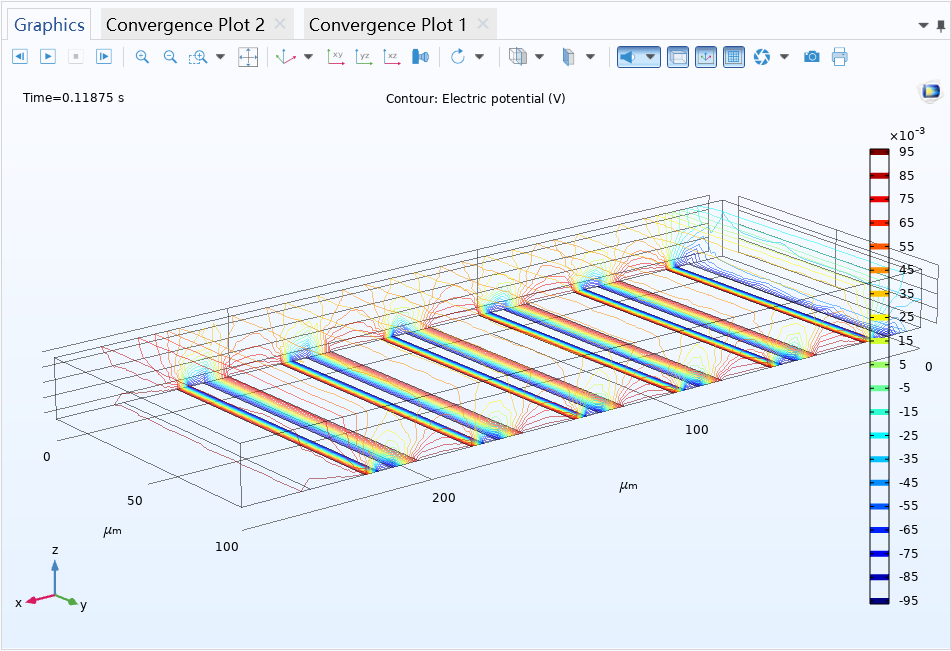
\includegraphics[width=0.8\textwidth]{9.png}
    \end{figure}
\end{frame}
\begin{frame}
    \begin{center}
        Thanks!
    \end{center}
\end{frame}
\end{document}